\documentclass[11pt]{article}
\usepackage{graphicx,fullpage}
\pagestyle{plain}
\headheight0in
\headsep0in
\topmargin -0.1in
\textheight 9.0in
\oddsidemargin -0.0in
\textwidth 6.5in
\baselineskip 3ex
\renewcommand\baselinestretch{1}
\parindent 0in
\parskip 0.05in
\def\bc{\begin{center}}
\def\ec{\end{center}}
\def\qskip{\vspace{1.5in}}
\def\qspace{\vspace{1.5in}}
\def\ans{\it ANSWER: }

\begin{document}
\begin{center}
{\bf Statistics 531/Econ 677, Winter 2009}
\end{center}
We investigate the monthly number mumps cases reported in New York City,
 from January 1928 to June 1972. 
During this period, before the introduction of a vaccine, mumps was a common childhood disease to which almost all children were exposed.
Because mumps displays a characteristic rash it is fairly easily diagnosed. Mumps is a reportable disease, meaning that doctors have  a legal obligation to report any cases they encounter.
This dataset therefore gives an opportunity to study disease transmission and maybe learn lessons relevant to diseases of current concern such as bird flu, SARS or HIV/AIDS.
The data, which we shall denote by $\{x_t,t=1,2,\dots\}$, are graphed in Fig.~\ref{fig:data}.


\begin{figure}[h]
\bc
%\vspace{-0.7cm}
\vspace{-1cm}
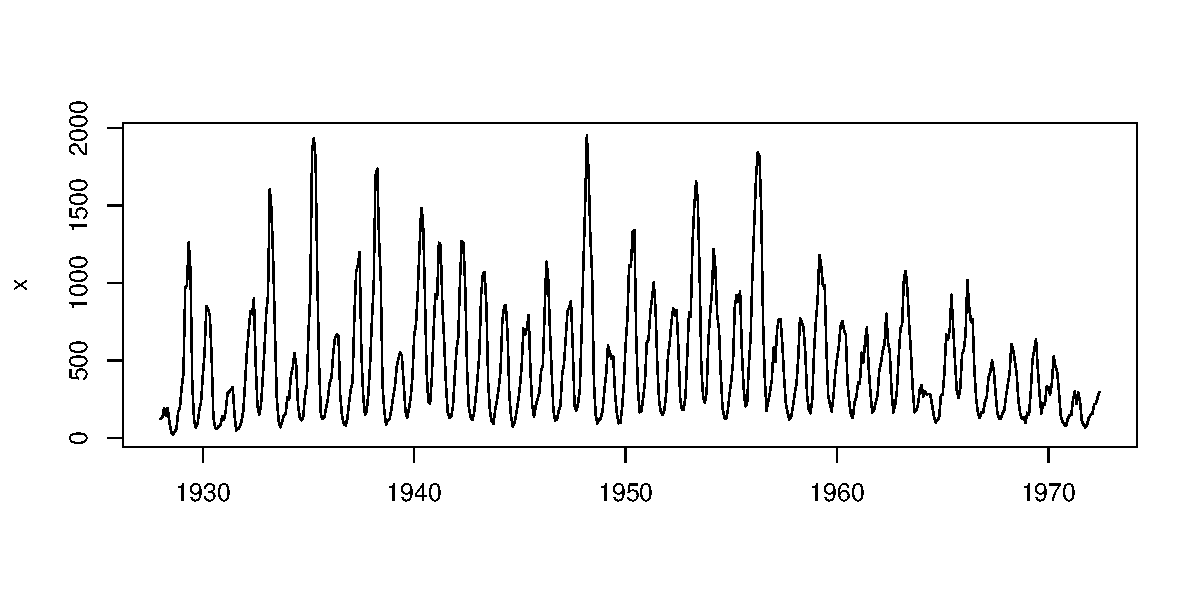
\includegraphics[width=6in]{mumps}
%\vspace{-0.5cm}
\vspace{-1.8cm}
\ec
\caption{Monthly mumps reports, $x_t$, in New York City from January 1928 to June 1972.}\label{fig:data}
\end{figure}



\noindent {\bf Section A. Spectral analysis}. We seek to interpret the estimated spectum in Fig.~\ref{fig:spec} and in particular the features labeled (1) through (5).


\begin{figure}[h]
\bc\vspace{-1cm}
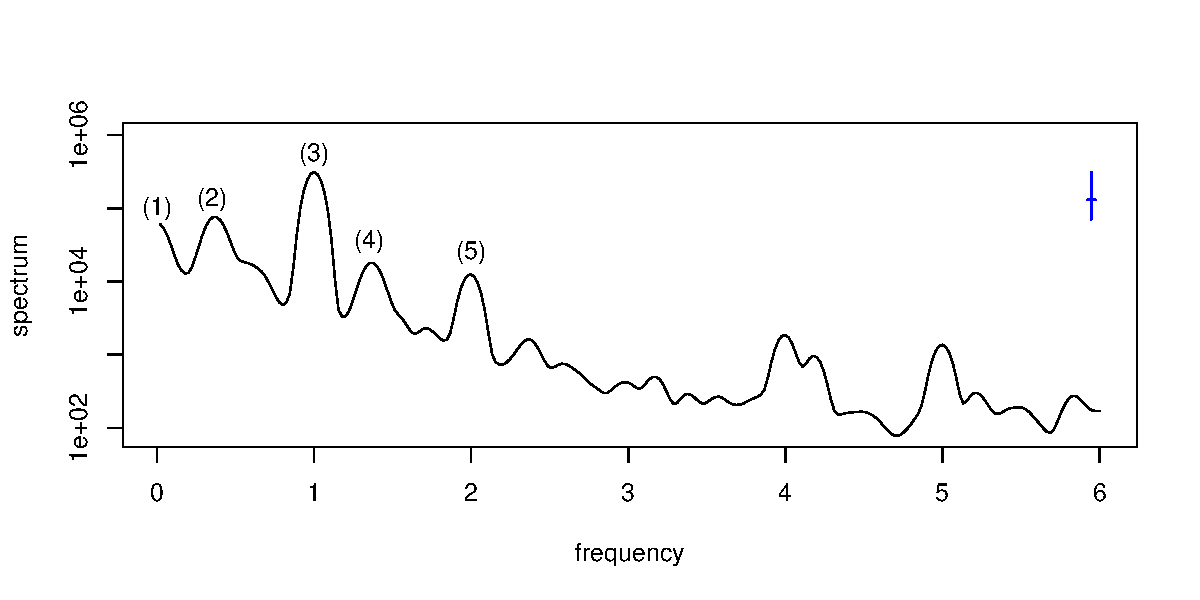
\includegraphics[width=6in,height=2.5in]{mumps-spec}
\ec\vspace{-1cm}
\caption{An estimated spectral density for $x_t$, calculated via \texttt{spectrum(x,spans=c(3,5,7))}.}\label{fig:spec}
\end{figure}

A1. [2 points] What are the units of frequency in Fig.~\ref{fig:spec}? Explain how you reach your answer.

{\ans Spectra are usually plotted up to the Nyquist frequency of 0.5 cycles/observation, which corresponds to 6 cycles/year for monthly data. The labe on the $x$-axis thus suggests that units are cycles/year. The large peak at frequency 1 confirms this, since we see from the data that there is a dominant anual cycle (e.g. ten peaks between 1940 and 1950).}


%\vspace{1in}

%\newpage

A2. [3 points] One might expect mumps to have annual seasonality. 
One might also expect mumps to have long term cycles as the
population of suscpetible children (those without immunity)
replenishes after previous outbreaks. 
%Is there evidence for this?
%Over what timespan? As part of your answer, 
Discuss the interpretation of the 5 spectral peaks labeled (1) through (5) in Fig.~\ref{fig:spec}. You do not have to discuss here whether these peaks are statistically significant, which is question A3 below.

{\ans (1) is low frequency variation, or trend. (2) is at $\approx 1/3$ cycles/year; these 3 year cycles could correspond to the replenishment of susceptible children suggested in the question. (3) is an annual cycle. (4) is at $\approx 1.3$ cycles/year (period of $\approx 0.8$yr) which is hard to interpret but could be a harmonic of (2). The  2 cycles/year peak in (5) is a seasonal effect---i.e., a harmonic of (3)---indicating that the seasonal oscillations are not sinusoidal; this might match the suggestion of slight double peaks in many of the epidemics.}

%\vspace{5in}

A3. [2 points] Comment on the statistical significance of these five peaks. You are not expected to present formal tests, but you should say what your opinion is and why.

{\ans Moving the crossbar to each point along the estimated spectrum gives pointwise 95\% confidence intervals. (3) is clearly significant. Most people felt that the confidence intervals for (1,2,4,5) also did not include the base of the peak, indicating significance. Borderline cases cannot be definitively answered by such an informal test.}

%\vspace{2in}

%\newpage

\noindent {\bf Section B. ARIMA analysis}. We try fitting an
$ARIMA(3,0,0)\times(0,1,1)_{12}$ model. Call this model M1. The output from {\texttt{M1=arima(x,order=c(3,0,0),seasonal=c(0,1,1))}} is
\vspace{-3mm}
\begin{verbatim}
         ar1      ar2      ar3     sma1
      1.2032  -0.3025  -0.0632  -0.8841
s.e.  0.0439   0.0674   0.0442   0.0231

sigma^2 estimated as 12881:  log likelihood = -3220.76,  aic = 6451.51
\end{verbatim}

Another possibility is to model %$y_t=\log(x_t)$, 
$\log(x_t)$, again using 
$ARIMA(3,0,0)\times(0,1,1)_{12}$. Call this model M2. The output from 
\texttt{M2=arima(log(x),order=c(3,0,0),seasonal=c(0,1,1))}
is
\vspace{-3mm}
\begin{verbatim}
         ar1     ar2      ar3     sma1
      0.9197  0.1577  -0.1710  -0.8080
s.e.  0.0434  0.0592   0.0438   0.0285

sigma^2 estimated as 0.03632:  log likelihood = 117.48,  aic = -224.96
\end{verbatim}

B1. [2 points] Can the above analysis determine whether a log
transformation is appropriate? Explain.

{\ans No. AIC values cannot be used to compare transformations of
the data. Similarly $\sigma^2$ values are not comparable. With
extra care, likelihoods can be transformed to be comparable.}

%\vspace{2in}

A table comparing AIC values for various
$ARIMA(i,0,j)\times(0,1,1)_{12}$ models for $\log(x_t)$ is given below:

\begin{tabular}{crrrrr}
AR $\setminus$ MA & 0 & 1 & 2& 3& 4\\
  0&        NA  &312.7628 &  92.7453  &-42.91403 &-131.8598\\
1& -213.9453 &-211.9458 &-224.4315 &-227.35447 &-225.5215\\
2& -211.9459 &-212.5350 &-236.8260 &-223.70594 &-224.7305\\
3& -224.9618 &-237.9834 &-236.1537 &-234.41349 &-232.4061\\
4& -229.8224 &-221.1222 &-236.4941 &-235.21621 &-239.7320\\
\end{tabular}

B2. [2 points] The software gave no error messages while computing this
table. Is there any reason to suspect that the numeric
maximization of the likelihood is less than adequate?

{\ans Yes. Adding 1 parameter can only increase AIC by 2. Compare
ARMA(3,1) with ARMA(4,1) and see this is violated. Note that, under the reasonable assumption that likelihood evaluation is adequate, the problem in this case appears to be with the maximization of ARMA(4,1) and should not necessarily discourage the selection of ARMA(3,1).}

%\qspace

%\newpage
B3. [4 points] Discuss briefly what you learn from the AIC table shown, in terms of developing a suitable model for these data.
Explain briefly why AIC may not be the only criterion
considered when selecting a model, and list some other analyses that you would carry out to determine and defent a choice of model.

{\ans AIC favors ARMA(3,1) and ARMA(4,4). The latter is a large model, and is on the boundary of those considered  in the table, so is not a good choice. One could penalize the likelihood differently, e.g. using
BIC. Simplicity may be particularly valuable if we want to
interpret parameters. Redundant models (or close to redundant)
are undesirable, whatever the AIC. If normality is seriously violated, AIC
may be untrustworthy. Similarly if there are problems with
numeric maximization of the likelihood, as diagnosed in B2 above.}

%\vspace{5in}

\noindent {\bf Section C. Diagnostic analysis}. Fig.~\ref{fig:diag} contains six diagnostic plots, three for each of models M1 and M2.

C1. [2 points] Explain carefully the meaning of the dashed line in sample
ACF plots produced by R, for example in Fig.~\ref{fig:diag}(a1). [Here, you are asked to explain the statistical method; later parts will ask you to interpret the results in the context of the data and models under investigation.]

{\ans If the data were Gaussian white noise then ACF at each lag would fall between the dotted lines with probability 95\%. This is often summarized (with some abuse of terminology) by saying that the dotted lines are a 95\% confidence interval for Gaussian white noise.}

%\vspace{2in}

%\newpage


\begin{figure}[h]\vspace{-0.5cm}
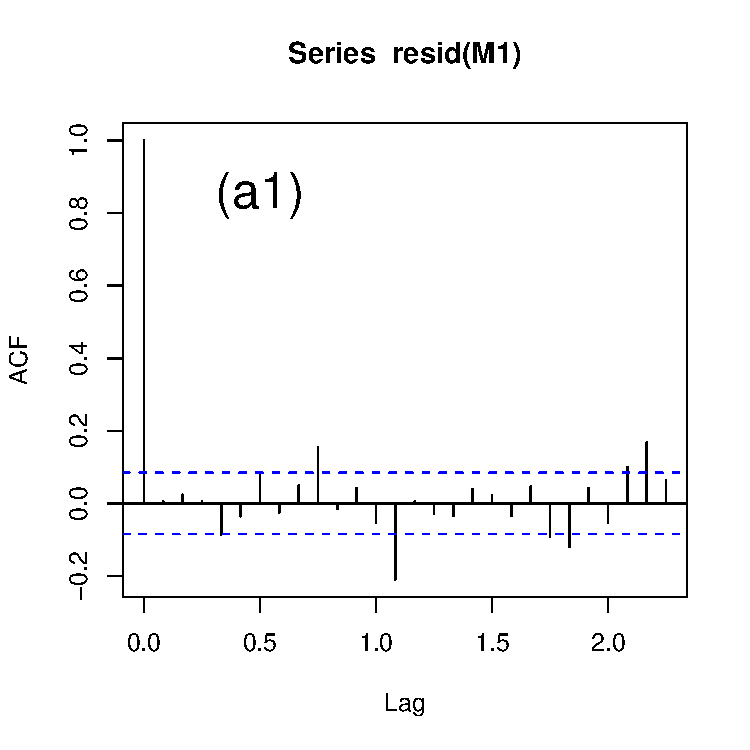
\includegraphics[width=3in,height=2.5in]{m1-resid}
\hfill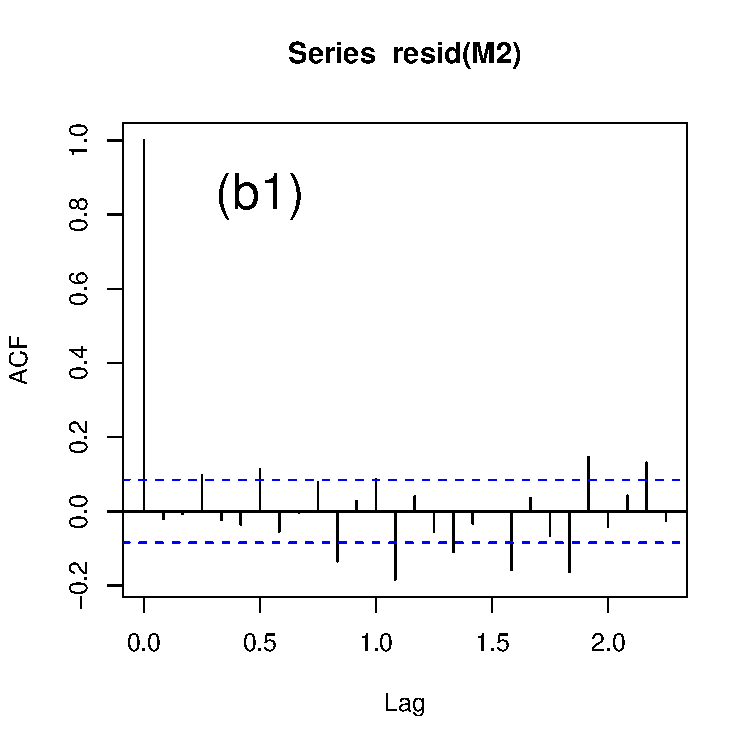
\includegraphics[width=3in,height=2.5in]{m2-resid}

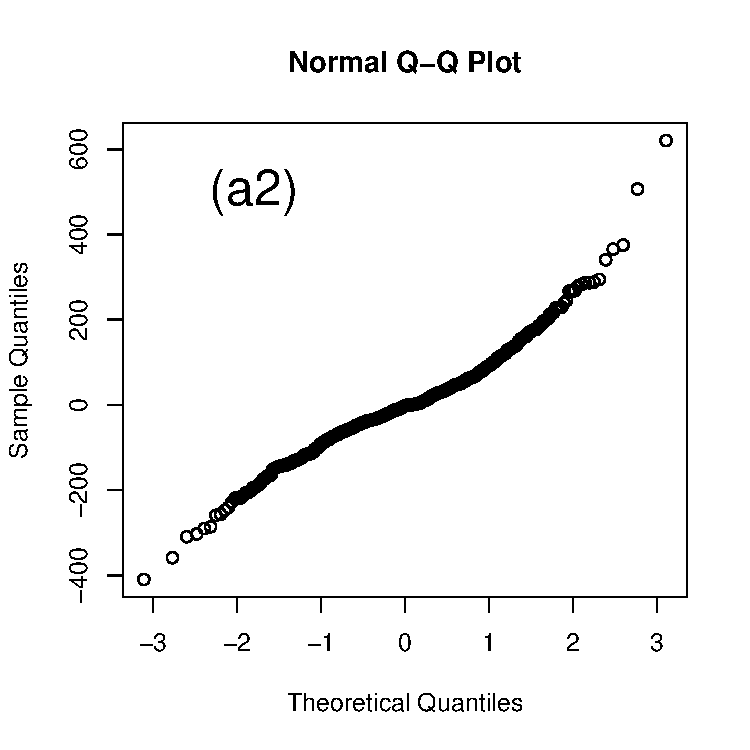
\includegraphics[width=3in,height=2.5in]{m1-qq}
\hfill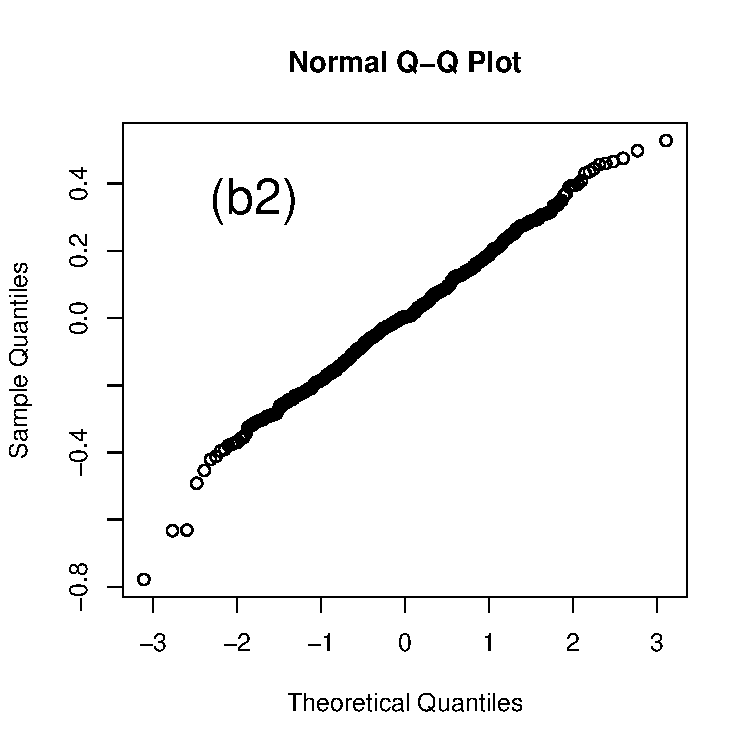
\includegraphics[width=3in,height=2.5in]{m2-qq}

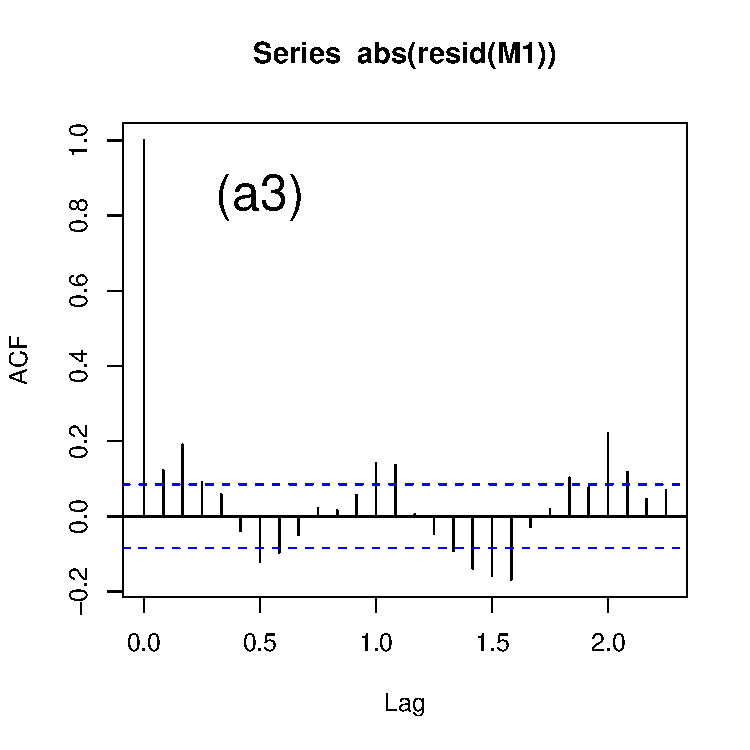
\includegraphics[width=3in,height=2.5in]{m1-resid2}
\hfill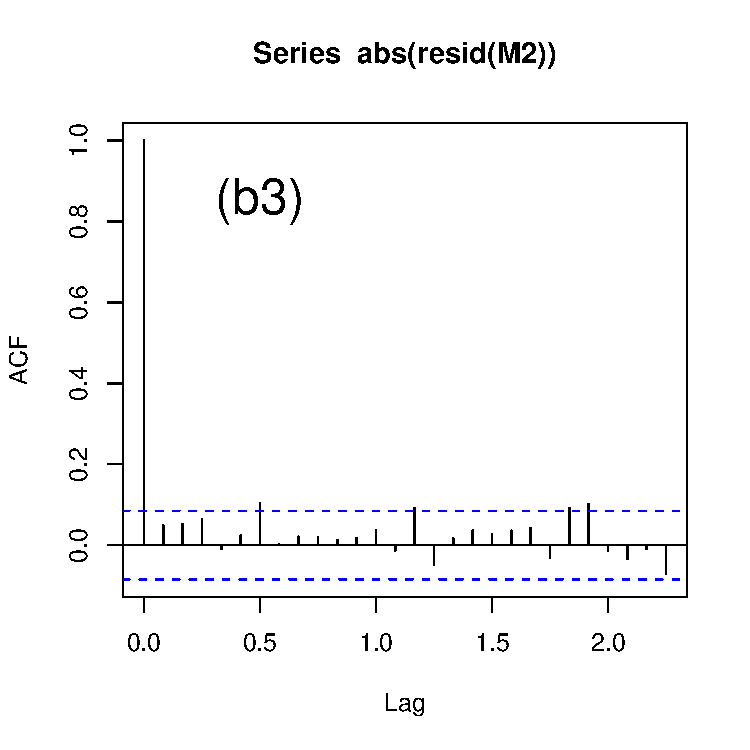
\includegraphics[width=3in,height=2.5in]{m2-resid2}

\caption{
Some diagnostic plots. (a1) and (a3) show the sample ACF
for the residuals and absolute values of the residuals
respectively for model M1. (a2) is a normal quantile plot of the residuals for M1.
(b1,b2,b3) are the equivalent diagnostic plots for M2.
}\label{fig:diag}
\end{figure}

%\newpage
%\clearpage

C2. [2 points] Compare (a1) and (b1) in Fig.~\ref{fig:diag}. What does this
tell you about models M1 and M2?

{\ans Both indicate mild deviation from white noise.}

%\qspace
%\vspace{2.5in}


C3. [2 points] Compare (a2) and (b2) in Fig.~\ref{fig:diag}. What does this
tell you about models M1 and M2?

{\ans (a2) shows long tails, at both ends. (b) shows less
deviation from normality, though still a long left tail.}

%\qspace
%\vspace{2.5in}

C4. [2 points] Compare (a3) and (b3) in Fig.~\ref{fig:diag}. What does this
tell you about models M1 and M2? In particular, what do you learn about the appropriateness of an assumption that the white noise process driving the ARIMA model is independent and identically distributed?

{\ans (a3) shows that the residuals with large absolute value for
M1 occur periodically. This is a deviation from the Gaussian
white noise hypothesis, for which the absolute values are also
uncorrelated. (b3) is consistent with   Gaussian
white noise.}

%\qspace
%\vspace{2.5in}

\end{document}
